\documentclass[9pt]{beamer}
\usetheme[progressbar=frametitle]{metropolis}
\usecolortheme{metropolis}
\usepackage{graphicx}
\usepackage{color}
\usepackage{amsmath, amscd, mathtools, stmaryrd}
\usepackage{empheq}
\usepackage[skip=2pt]{caption}
\usepackage{tcolorbox}
\usepackage{minted}

\definecolor{mDarkBrown}{HTML}{604c38}
\definecolor{mDarkTeal}{HTML}{23373b}
\definecolor{mLightBrown}{HTML}{EB811B}
\definecolor{mLightGreen}{HTML}{14B03D}
\definecolor{maroon}{rgb}{0.76, 0.13, 0.28}
\definecolor{orange}{HTML}{b96500}

\renewcommand\vec{\mathbf}

\newenvironment{variableblock}[3]{%
	\setbeamercolor{block body}{#2}
	\setbeamercolor{block title}{#3}
	\begin{block}{#1}}{\end{block}}

% For diagrams
\usepackage{tikz}
\usetikzlibrary{matrix, calc}

\title{A multigrid method with non-nested space hierarchies: applications with hybridization}
\date{September 27, 2019}
\author{\textbf{\underline{Thomas Gibson}}\inst{1,3}\\
	Eike M\"uller\inst{2} and Jack Betteridge\inst{2}}
\institute{\textbf{Firedrake 2019} \and
	\inst{1} Department of Mathematics, Imperial College London \\
	\inst{2} Department of Mathematics, University of Bath \\
	\inst{3}\texttt{\underline{t.gibson15@imperial.ac.uk}}}

\begin{document}

\maketitle

\begin{frame}[c]{Motivation}

\begin{variableblock}{Challenges in numerical weather prediction}{bg=white,fg=mDarkTeal}{bg=mDarkTeal,fg=white}
	\vspace{10pt}
	\begin{columns}
		\begin{column}{0.5\textwidth}
			\centering
			\includegraphics[width=\linewidth]{figures/globalweatherforecast20192-1}
		\end{column}
		\hspace{-20pt}\begin{column}{0.5\textwidth}
			\begin{itemize}
				\item Substantial increase in global resolution:
				$25\mathrm{km} \rightarrow 5-8\mathrm{km}$
				\item 5 day forecasts $\implies$ model runtime
				needs to be under an hour!
				\item Semi-implicit time-integrators
				$\implies$ \textcolor{maroon}{Need scalable solvers!}
			\end{itemize}
		\end{column}
	\end{columns}
\end{variableblock}
\begin{columns}
	\begin{column}{0.5\textwidth}
		Requires repeatedly solving complex PDE systems:
		\begin{empheq}[box=\fbox]{equation*}
		\begin{bmatrix}
		M_1 & B^T & Q^T \\
		B & M_2 & 0 \\
		Q & 0 & M_3
		\end{bmatrix}
		\begin{Bmatrix}
		\vec{u} \\ p \\ \theta
		\end{Bmatrix} =
		\begin{Bmatrix}
		R_1 \\ R_2 \\ R_3
		\end{Bmatrix}
		\end{empheq}
	\end{column}
	\hspace{-20pt}\begin{column}{0.5\textwidth}
		\centering
		\includegraphics[width=\linewidth]{figures/hurricane}
	\end{column}
\end{columns}
\end{frame}

%\begin{frame}[c]{Motivation}
%\begin{columns}
%	\begin{column}{0.5\textwidth}
%		Other applications with similar PDE structures:
%		\begin{itemize}
%			\item Global ocean circulation
%			\item Storm-surge / coastal ocean modeling
%			\item Sub-surface and reservoir modeling
%			\item ... Many more!
%		\end{itemize}
%	\centering
%	\includegraphics[width=\linewidth]{figures/subsurface}
%	\end{column}
%	\hspace{-20pt}\begin{column}{0.5\textwidth}
%		\centering
%		\includegraphics[width=\linewidth]{figures/ike_ss}%
%		\vspace{20pt}
%		\includegraphics[width=\linewidth]{figures/conveyor}
%	\end{column}
%\end{columns}
%\end{frame}

\begin{frame}[c]{Numerics for weather and oceans}
	Traditional codes typically use C-grid finite differences
	on structured grids
	\begin{columns}
		\begin{column}{0.5\textwidth}
			\begin{center}
				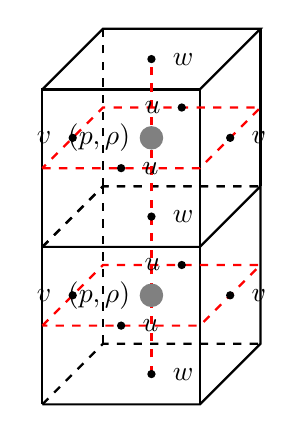
\begin{tikzpicture}[thick, scale=0.5]
					%%
\coordinate (1) at (0,0,4);
\coordinate (2) at (4,0,4);
\coordinate (3) at (4,0,0);
\coordinate (4) at (0,0,0);
\coordinate (5) at (0,4,4);
\coordinate (6) at (4,4,4);
\coordinate (7) at (4,4,0);
\coordinate (8) at (0,4,0);
\coordinate (9) at (0,8,0);
\coordinate (10) at (4,8,0);
\coordinate (11) at (4,8,4);
\coordinate (12) at (0,8,4);

\draw (1) -- (2) -- (3) -- (7) --(6) -- (5);
\draw[dashed] (5) -- (8) -- (7);
\draw (1)--(5);
\draw (2)--(6);
\draw[dashed] (1)--(4) -- (3);
\draw[dashed] (4)--(8);
\draw[dashed] (5) -- (8) -- (7);
\draw (5) -- (12) -- (11) -- (6);
\draw (12) -- (9) -- (10) -- (11);
\draw (10) -- (7);
\draw[dashed] (8) -- (9);

\coordinate (u11) at ($(1)!.5!(6)$);
\coordinate (u12) at ($(4)!.5!(7)$);
\coordinate (v11) at ($(1)!.5!(8)$);
\coordinate (v12) at ($(2)!.5!(7)$);
\coordinate (w00) at ($(1)!.5!(3)$);
\coordinate (w11) at ($(5)!.5!(7)$);
\coordinate (w22) at ($(12)!.5!(10)$);
\coordinate (p1) at ($(1)!.5!(7)$);
\coordinate (p2) at ($(5)!.5!(10)$);
\coordinate (u21) at ($(5)!.5!(11)$);
\coordinate (u22) at ($(8)!.5!(10)$);
\coordinate (v21) at ($(5)!.5!(9)$);
\coordinate (v22) at ($(6)!.5!(10)$);

\coordinate (a1) at ($(1)!.5!(5)$);
\coordinate (b1) at ($(4)!.5!(8)$);
\coordinate (c1) at ($(2)!.5!(6)$);
\coordinate (d1) at ($(3)!.5!(7)$);

\coordinate (a2) at ($(5)!.5!(12)$);
\coordinate (b2) at ($(6)!.5!(11)$);
\coordinate (c2) at ($(7)!.5!(10)$);
\coordinate (d2) at ($(8)!.5!(9)$);

%\foreach \i in {1, ..., 12}
%\fill (\i) node [
%circle, inner sep=0pt, minimum size=3pt
%] {\i};
\draw[dashed, red] (a1)-- (b1) -- (d1) -- (c1) -- (a1);
\draw[dashed, red] (a2)-- (b2) -- (c2) -- (d2) -- (a2);
\draw[dashed, red] (w00) -- (w22);

\foreach \i in {u11, u12, v11, v12, w00, w11, w22, u21, u22, v21, v22}
\fill (\i) node [
circle, fill=black, inner sep=0pt, minimum size=3pt
] {};

\foreach \i in {p1, p2}
\fill (\i) node [
circle, double, fill=gray, inner sep=3pt, minimum size=5pt,
] {};

\node[right=4pt] at (w00) {$w$};
\node[right=4pt] at (w11) {$w$};
\node[right=4pt] at (w22) {$w$};

\node[left=4pt] at (p2) {$(p, \rho)$};
\node[left=4pt] at (p1) {$(p, \rho)$};

\node[left=4pt] at (v21) {$v$};
\node[left=4pt] at (v11) {$v$};
\node[right=4pt] at (v12) {$v$};
\node[right=4pt] at (v22) {$v$};

\node[left=4pt] at (u12) {$u$};
\node[left=4pt] at (u22) {$u$};
\node[right=4pt] at (u21) {$u$};
\node[right=4pt] at (u11) {$u$};
				\end{tikzpicture}\\
				Arakawa C-grid in 3D
			\end{center}
		\end{column}
		\hspace{-20pt}\begin{column}{0.5\textwidth}
			\begin{center}
				\begin{tikzpicture}[thick, scale=0.5]
					\input{latlong/latlong}
				\end{tikzpicture}
				``Lat-long" horizontal mesh	
			\end{center}
		\end{column}
	\end{columns}
	The mixed system is avoided by eliminating into an
	\emph{elliptic} pressure equation:
	\begin{empheq}[box=\fbox]{equation*}
		-\omega\left\lbrack \nabla^2_\mathcal{S} \Pi + \frac{\lambda^2}{r^2}
		\frac{\partial }{\partial r}\left(r^2\frac{\partial \Pi}{\partial r}\right)
		\right\rbrack + \Pi = ...
	\end{empheq}
\end{frame}

\begin{frame}[c]{Towards finite elements}
	Finite element alternatives are popular:
	\begin{itemize}
		\item Discontinuous Galerkin methods
		\item \textcolor{maroon}{Mixed (``compatible") methods} (more recent)
		\begin{itemize}
			\item Raviart-Thomas / Brezzi-Douglas-Marini mixed methods
		\end{itemize}
	\end{itemize}
because:
	\begin{columns}
	\begin{column}{0.5\textwidth}
		\begin{itemize}
			\item methods are mesh-agnostic (avoids the pole problem)
			\item In the case of compatible finite element methods,
			preserved the mimetic properties of the C-grid.
			\begin{itemize}
				\item Calculus identities are discretely preserved:
				\begin{align*}
					\nabla\cdot(a\vec{b}) &= \vec{b}\cdot\nabla a + a\nabla\cdot\vec{b}\\
					\nabla\times\nabla a &= 0 \\
					\nabla\cdot\nabla\times\vec{b} &= 0
				\end{align*}
			\end{itemize}
		\end{itemize}
	\end{column}
	\hspace{-20pt}\begin{column}{0.5\textwidth}
		\begin{center}
			\vspace{-20pt}\includegraphics[width=\textwidth]{figures/cubed_sphere_mesh}
			quasi-uniform cubed-sphere mesh
		\end{center}
	\end{column}
\end{columns}
\end{frame}

\begin{frame}[c]{Lowest-order mixed finite elements (http://femtable.org/)}
	\vspace{-2.5mm}
	\begin{center}
		\begin{minipage}{0.5\textwidth}
			\centering
			\begin{figure}
				\includegraphics[width=0.5\linewidth]{figures/Q1_interval}
				\caption*{Continuous interval}
			\end{figure}
		\end{minipage}%
		\begin{minipage}{0.5\textwidth}
			\centering
			\begin{figure}
				\includegraphics[width=0.5\linewidth]{figures/dQ0_interval}
				\caption*{Discontinuous interval}
			\end{figure}
		\end{minipage}
	\end{center}%
	\begin{center}\vspace{-5mm}
		\begin{minipage}{0.33\textwidth}
			\centering
			\begin{figure}
				\includegraphics[width=0.7\linewidth]{figures/Q1_quadrilateral}
				\caption*{Cont. quad}
			\end{figure}
		\end{minipage}%
		\begin{minipage}{0.33\textwidth}
			\centering
			\begin{figure}
				\includegraphics[width=0.59\linewidth]{figures/rtcf1}
				\caption*{``Velocity'' element}
			\end{figure}
		\end{minipage}%
		\begin{minipage}{0.33\textwidth}
			\centering
			\begin{figure}
				\includegraphics[width=0.7\linewidth]{figures/dQ0_quadrilateral}
				\caption*{Discont. quad}
			\end{figure}
		\end{minipage}
	\end{center}%
	\begin{center}\vspace{-2.5mm}
		\begin{figure}
			\centering
			\begin{minipage}{0.5\textwidth}
				\centering
				\includegraphics[width=0.475\linewidth]{figures/w0}%
				\includegraphics[width=0.5\linewidth]{figures/w1}
				\captionof*{figure}{$\mathbb{W}_0$ \quad\quad\quad\quad\quad\quad $\mathbb{W}_1$}
			\end{minipage}%
			\begin{minipage}{0.5\textwidth}\vspace{1mm}
				\centering
				\includegraphics[width=0.5\linewidth]{figures/w2}%
				\includegraphics[width=0.5\linewidth]{figures/w3}
				\captionof*{figure}{$\mathbb{W}_2$ \quad\quad\quad\quad\quad\quad $\mathbb{W}_3$}
			\end{minipage}
		\end{figure}
	\end{center}
\end{frame}

\begin{frame}[c]{Illustrating the problem: a simple model}
\begin{columns}
	\begin{column}{0.5\textwidth}
		Linear shallow water equations (no rotation, mean depth $H=1$):
		\begin{align*}
			\frac{\partial \vec{u}}{\partial t} + g\nabla h &= 0,\\
			\frac{\partial h}{\partial t} + \nabla\cdot\vec{u} &= 0.
		\end{align*}
		Compatible finite element discretization (lowest order):
		find $\vec{u} \in RT_0$, $h \in DG_0$:
		\begin{empheq}[box=\fbox]{align*}
			\textcolor{maroon}{\int_{\Omega} \vec{w}\cdot\frac{\partial \vec{u}}{\partial t}
				\mathrm{d}x} - g\int_{\Omega}h\nabla\cdot\vec{w}\mathrm{d}x &= 0,\\
			\int_{\Omega}\phi \frac{\partial h}{\partial t}\mathrm{d}x
			+ \int_{\Omega}\phi\nabla\cdot\vec{u}\mathrm{d}x &= 0,
		\end{empheq}
		$\forall \vec{w}, \phi \in RT_0 \times DG_0$.
	\end{column}
	\hspace{-20pt}\begin{column}{0.5\textwidth}
		Discretizing (implicitly) in time requires the solution
		of the saddle-point system:
		\begin{empheq}[box=\fbox]{equation*}
		\begin{bmatrix}
		\textcolor{maroon}{M_1} & -gB^T \\
		B & M_2
		\end{bmatrix}
		\begin{Bmatrix}
		\vec{u}^n \\ h^n
		\end{Bmatrix}
		= \begin{Bmatrix}
		R_1 \\ R_2
		\end{Bmatrix}
		\end{empheq}
		\begin{variableblock}{Elliptic equation}{bg=white,fg=mDarkTeal}{bg=mDarkTeal,fg=white}
			An elliptic problem can be obtained by eliminating
			$\vec{u}^n$:
			\begin{equation*}
				\left(M_2 + gB \textcolor{maroon}{M_1^{-1}} B^T\right)h^n = ...
			\end{equation*}
		\end{variableblock}
		\begin{variableblock}{Problem!}{bg=white,fg=mDarkTeal}{bg=mDarkTeal,fg=white}
			Not practical in real applications because of the dense
			(globally) inverse $\textcolor{maroon}{M_1^{-1}}$.
		\end{variableblock}
	\end{column}
\end{columns}
\end{frame}

\begin{frame}[c]{Global sparsity pattern}
	\begin{figure}
		\centering
		\includegraphics[width=\textwidth]{figures/global_mixed_sparsity}
	\end{figure}
\end{frame}

\begin{frame}[c]{Hybridization of the mixed method}
	\vspace{10pt}\begin{columns}
		\begin{column}{0.5\textwidth}
			Discrete \emph{hybridizable} problem:
			find $\vec{u}^n \in RT^d_0$, $h^n \in DG_0$, $\lambda \in T_0$:
			\begin{align*}
			\textcolor{maroon}{\int_{\Omega} \vec{w}\cdot\vec{u}^n
				\mathrm{d}x} - g\alpha\Delta t\int_{\Omega}h^n\nabla\cdot\vec{w}\mathrm{d}x\\
			+ \textcolor{orange}{\sum_{K}g\alpha\Delta t\int_{\partial K}\lambda\vec{w}\cdot\vec{n}\mathrm{d}S} &= ...,\\
			\int_{\Omega}\phi h^n\mathrm{d}x
			+ \alpha\Delta t\int_{\Omega}\phi\nabla\cdot\vec{u}^n\mathrm{d}x &= ...,\\
			\textcolor{orange}{\sum_{K}\int_{\partial K}\gamma\vec{u}\cdot\vec{n}\mathrm{d}S} &= 0
			\end{align*}
			$\forall \vec{w}, \phi, \gamma \in RT_0 \times DG_0 \times T_0$.
			\begin{center}
				\includegraphics[width=0.75\linewidth]{figures/w2b_w2t}\\
				$RT_1^d$ and $T_1$ on quadrilaterals
			\end{center}
		\end{column}
		\hspace{-20pt}\begin{column}{0.5\textwidth}
			\begin{center}
				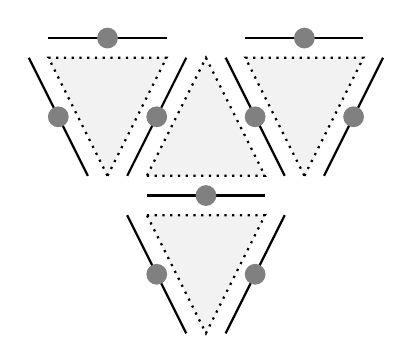
\begin{tikzpicture}[thick, scale=0.5]
					%%
% middle
\coordinate (v1) at (0, 0);
\coordinate (v2) at (3, 0);
\coordinate (v3) at (1.5, 3);

% left
\coordinate (v4) at (-1, 0);
\coordinate (v5) at (0.5, 3);
\coordinate (v6) at (-2.5, 3);

% right
\coordinate (v7) at (4, 0);
\coordinate (v8) at (5.5, 3);
\coordinate (v9) at (2.5, 3);

% bottom
\coordinate (v10) at (0, -1);
\coordinate (v11) at (3, -1);
\coordinate (v12) at (1.5, -4);

\draw[fill=gray!10, dotted] (v1) -- (v2) -- (v3) -- cycle;
\draw[fill=gray!10, dotted] (v4) -- (v5) -- (v6) -- cycle;
\draw[fill=gray!10, dotted] (v7) -- (v8) -- (v9) -- cycle;
\draw[fill=gray!10, dotted] (v10) -- (v11) -- (v12) -- cycle;

% internal edges
\coordinate (v14) at ($(v1)!.5!(v4)$);
\coordinate (v35) at ($(v3)!.5!(v5)$);
\coordinate (v110) at ($(v1)!.5!(v10)$);
\coordinate (v211) at ($(v2)!.5!(v11)$);
\coordinate (v27) at ($(v2)!.5!(v7)$);
\coordinate (v39) at ($(v3)!.5!(v9)$);

\draw (v14) -- (v35);
\draw (v110) -- (v211);
\draw (v27) -- (v39);

% external edges
\coordinate (v5e1) at (0.5, 3.5);
\coordinate (v6e1) at (-2.5, 3.5);
\coordinate (v6e2) at (-3, 3);
\coordinate (v4e1) at (-1.5, 0);
\coordinate (v9e1) at (2.5, 3.5);
\coordinate (v8e1) at (5.5, 3.5);
\coordinate (v8e2) at (6, 3);
\coordinate (v7e1) at (4.5, 0);
\coordinate (v10e1) at (-0.5, -1);
\coordinate (v11e1) at (3.5, -1);
\coordinate (v12e1) at (1, -4);
\coordinate (v12e2) at (2, -4);

\draw (v5e1) -- (v6e1);
\draw (v6e2) -- (v4e1);
\draw (v8e1) -- (v9e1);
\draw (v8e2) -- (v7e1);
\draw (v10e1) -- (v12e1);
\draw (v11e1) -- (v12e2);

% global trace dofs
\coordinate (t1) at ($(v14)!.5!(v35)$);
\coordinate (t2) at ($(v110)!.5!(v211)$);
\coordinate (t3) at ($(v27)!.5!(v39)$);
\coordinate (t4) at ($(v5e1)!.5!(v6e1)$);
\coordinate (t5) at ($(v6e2)!.5!(v4e1)$);
\coordinate (t6) at ($(v8e1)!.5!(v9e1)$);
\coordinate (t7) at ($(v8e2)!.5!(v7e1)$);
\coordinate (t8) at ($(v10e1)!.5!(v12e1)$);
\coordinate (t9) at ($(v11e1)!.5!(v12e2)$);

\foreach \i in {t1, t2, t3, t4, t5, t6, t7, t8, t9}
\fill (\i) node [
circle, fill=gray, inner sep=0pt, minimum size=7.5pt
] {}; % Leave blank so numbers don't appear
				\end{tikzpicture}\\
				Global trace space $T_0$ on triangles
			\end{center}
			\begin{variableblock}{Matrix system}{bg=white,fg=mDarkTeal}{bg=mDarkTeal,fg=white}
				\begin{equation*}
					\begin{bmatrix}
					\textcolor{maroon}{\tilde{M}_1} & -g\tilde{B}^T & \textcolor{orange}{K^T} \\
					\tilde{B} & M_2 & 0 \\
					\textcolor{orange}{K} & 0 & 0
					\end{bmatrix}
					\begin{Bmatrix}
					\vec{u}^n \\ h^n \\ \lambda
					\end{Bmatrix}
					= \begin{Bmatrix}
					\tilde{R}_1 \\ R_2 \\ 0
					\end{Bmatrix}
				\end{equation*}
			\end{variableblock}
		\end{column}
	\end{columns}
\end{frame}

\begin{frame}[c]{Global sparsity pattern (hybridizable)}
	\begin{figure}
		\centering
		\includegraphics[width=\textwidth]{figures/global_hybridized_sparsity}
	\end{figure}
\end{frame}

\begin{frame}[c]{Eliminating and recovering velocity / depth \emph{locally}}
	A \emph{sparse} elliptic equation for $\lambda$
	can be obtained
	\begin{equation*}
		S\lambda = E,
	\end{equation*}
	where $S$ and $E$ are obtained via \emph{local} static
	condensation:
	\begin{align*}
		S &= \begin{bmatrix}
		K & 0
		\end{bmatrix}
		\begin{bmatrix}
		\tilde{M}_1 & -g\tilde{B}^T \\
		\tilde{B} & M_2
		\end{bmatrix}^{-1}
		\begin{bmatrix}
		K^T \\ 0
		\end{bmatrix}, \\
		E &= \begin{bmatrix}
		K & 0
		\end{bmatrix}
		\begin{bmatrix}
		\tilde{M}_1 & -g\tilde{B}^T \\
		\tilde{B} & M_2
		\end{bmatrix}^{-1}
		\begin{Bmatrix}
		\tilde{R}_1 \\ R_2
		\end{Bmatrix}
	\end{align*}
	$\vec{u}^n$ and $h^n$ can be recovered locally:
	\begin{equation*}
		\begin{Bmatrix}
		\vec{u}^n \\ h^n
		\end{Bmatrix}
		= \begin{bmatrix}
		\tilde{M}_1 & -g\tilde{B}^T \\
		\tilde{B} & M_2
		\end{bmatrix}^{-1}
		\left(
		\begin{Bmatrix}
		\tilde{R}_1 \\ R_2
		\end{Bmatrix} -
		\begin{bmatrix}
		K^T \\ 0
		\end{bmatrix}
		\lambda
		\right)
	\end{equation*}
	\textcolor{maroon}{What about solvers for $S\lambda = E$?}
\end{frame}

\begin{frame}[c]{Solving for $\lambda$}
	\begin{equation*}\label{eq:trace}
	S\lambda = E
	\end{equation*}
	\vspace{-10pt}\begin{columns}
	\begin{column}{0.5\textwidth}
				\begin{variableblock}{What we know}{bg=white,fg=mDarkTeal}{bg=mDarkTeal,fg=white}
		\begin{itemize}
			\item $\lambda$ is an approximation of $h$ on
			the edges/faces of the mesh
			\item $S$ is spectrally similar to
			the Schur-complement from the original
			(unhybridized) system
			\textcolor{maroon}{(Gopolakrishnan, 2003)}
			\item $\lambda$ is the unique solution to
			an elliptic variational problem
			\textcolor{maroon}{(Cockburn, 2004)}:
			\begin{equation*}
				s(\lambda,\gamma) = e(\gamma), \forall \gamma \in T_k
			\end{equation*}
			\item S is positive definite;
			\begin{itemize}
				\item SPD if rotation is not included
			\end{itemize}
		\end{itemize}
		\end{variableblock}
	\end{column}
	\begin{column}{0.5\textwidth}
		\begin{tcolorbox}[width=\linewidth,
			%%frame hidden,
			left=0pt,
			right=0pt,
			top=2pt,
			]%%
			This \emph{screams} multigrid. But:
			\begin{itemize}
				\item Geometric multigrid directly on the
				trace system?
			\end{itemize}
		\end{tcolorbox}
	\begin{center}
		\includegraphics[width=\linewidth]{figures/hybrid-mesh}
	\end{center}
	Mesh hierarchy on $\mathcal{E}_h$ vs $\mathcal{T}_h$? Smoothers?
	\end{column}
\end{columns}
\end{frame}

\begin{frame}[c]{(Geometric) Multigrid: a (very) quick overview}
	\begin{center}
		\includegraphics[width=\linewidth]{figures/multigrid}
	\end{center}
\vspace{-10pt}\begin{itemize}
		\item Restriction operator: $R_{2h}$ moves data from
		fine to coarse ($h \rightarrow 2h$)
		\item Prolongation operator: $P_{h}$ moves data from coarse to fine ($2h \rightarrow h$).
		\item \textcolor{maroon}{Very important: smoothers $S$}
		(Jacobi/Gauss-Seidel/Successive over-relaxation (SOR)/Richardson)
		\item Direct down-up traversal of the grid hierarchy is
		called a \textcolor{maroon}{\emph{V-cycle}}.
	\end{itemize}
\end{frame}

%\begin{frame}[c]{Multigrid V-cycle algorithm}
%	Want to solve $A_h u = b_h$ on $\mathcal{T}_h$. For
%	some initial guess to $u$, $v_h$, we define
%	\begin{equation*}
%	v_h \leftarrow MGV(v_h, b_h, p, q)
%	\end{equation*}
%	with the following steps.
%	\begin{itemize}
%		\item[IF]: $h$ is the coarsest level:
%		\begin{equation*}
%			v_h = A_h^{-1}b_h
%		\end{equation*}
%		\item[ELSE]:
%		\begin{enumerate}
%			\item (Pre-smooth): Apply smoother
%			$v_h \leftarrow S(A_h, v_h, b_h)$ $p$ times using
%			initial guess $v_h$.
%			\item (Restrict residual): $r_{2h} = R_{2h}(b_h - A_h v_h)$.
%			\item $\epsilon_{2h} \leftarrow MGV(0, r_{2h}, p, q)$
%			\item (Prolong coarse grid error):
%			$v_h \leftarrow v_h + P_h\epsilon_{2h}$.
%			\item (Post-smooth): Apply smoother $v_h \leftarrow S(A_h, v_h, b_h)$ $q$ times.
%		\end{enumerate}
%	\end{itemize}
%\end{frame}

\begin{frame}[c]{Multigrid operators for $H^1$ finite elements}
	\begin{columns}
	\begin{column}{0.5\textwidth}
		\begin{tcolorbox}[colback=blue!5!white,colframe=mDarkTeal,title=$H^1$ (elliptic) problem]
			Find $p \in V_h(\mathcal{T}_h)
			\subset H^1(\mathcal{T}_h)$ such that
			\begin{equation*}
			a(p, q) = L(q), \forall p \in V_h.
			\end{equation*}
		\end{tcolorbox}
	Traditional MG methods construct a
	hierarchy: $\mathcal{T}_{1}, \cdots,
	\mathcal{T}_J \equiv \mathcal{T}_h$, with
	\begin{equation*}
		V_{1} \subset \cdots \subset V_J \equiv V_h,
	\end{equation*}
	With grid operators
	\begin{equation*}
		\left(A_j \phi, \psi\right)_k \equiv
		a(\phi, \psi), \forall\phi,\psi \in V_{j},
	\end{equation*}
	\end{column}
	\begin{column}{0.5\textwidth}
		\begin{tcolorbox}[title=Prolongation]
			Typically taken to be the natural injection
			operator: $P_{j}: V_{j-1} \rightarrow V_{j}$
			\begin{equation*}
				P_j \phi = \phi, \forall \phi \in V_{j-1}
			\end{equation*}
		\end{tcolorbox}
			\begin{tcolorbox}[colback=blue!5!white,colframe=mDarkTeal,title=Restriction]
				Restriction is the adjoint of prolongation
				w.r.t the inner products $(\cdot, \cdot)_j$ and
				$(\cdot, \cdot)_{j-1}$:
		\begin{equation*}
		(P_{j}\phi, \psi)_{j} = (\phi, R_{j-1}\psi)_{j-1},
		\end{equation*}
		$\forall \phi \in V_{j-1}$, $\psi \in V_j$.
	\end{tcolorbox}
	\end{column}
\end{columns}
\end{frame}

\begin{frame}[c]{Back to hybridization}
\begin{tcolorbox}[title=Mixed Poisson example (Cockburn and
	Gopalakrishnan 2004)]
	Find $\vec{u} \in U^d_h$, $p \in V_h$,
	$\lambda \in T_h$ such that
	\begin{align*}
	\int_{\mathcal{T}_h}\vec{w}\cdot\vec{u}\mathrm{d}x
	- \int_{\mathcal{T}_h}p\nabla\cdot\vec{w}\mathrm{d}x
	+ \sum_K \int_{\partial K}\lambda\vec{w}\cdot\vec{n}\mathrm{d}S &= 0,\\
	\int_{\mathcal{T}_h}\phi\nabla\cdot\vec{u}\mathrm{d}x &=
	\int_{\mathcal{T}_h} f\phi\mathrm{d}x,\\
	\sum_K \int_{\partial K}\gamma\vec{u}\cdot\vec{n}\mathrm{d}S &= 0,
	\end{align*}
	for all $\vec{w},\phi,\gamma$. The solutions have the form:
	$\vec{u} = \vec{Q}\lambda + \vec{Q}f$, $p = U\lambda + Uf$,
	where
\end{tcolorbox}
\begin{columns}
	\begin{column}{0.5\textwidth}
	\begin{tcolorbox}[colback=blue!5!white,colframe=mDarkTeal]
		$\vec{Q}\lambda$ and $U\lambda$ are contributions
		of the solutions determined by $\lambda$:
		\begin{equation*}
		\begin{bmatrix}
		A & -B^T \\
		B & 0
		\end{bmatrix}
		\begin{Bmatrix}
		\vec{Q}\lambda \\
			U\lambda
		\end{Bmatrix} =
		\begin{Bmatrix}
		-K^T\lambda \\ 0
		\end{Bmatrix}
		\end{equation*}
	\end{tcolorbox}
	\end{column}
	\begin{column}{0.5\textwidth}
	\begin{tcolorbox}[colback=blue!5!white,colframe=mDarkTeal]
	$\vec{Q}f$ and $Uf$ are contributions
	determined by the source:
	\begin{equation*}
	\begin{bmatrix}
	A & -B^T \\
	B & 0
	\end{bmatrix}
	\begin{Bmatrix}
	\vec{Q}f \\
	Uf
	\end{Bmatrix} =
	\begin{Bmatrix}
	 0 \\ f
	\end{Bmatrix}
	\end{equation*}
	\end{tcolorbox}	
	\end{column}
\end{columns}
\end{frame}

\begin{frame}[c]{Variational problem for $\lambda$}
	\begin{tcolorbox}[colback=blue!5!white,colframe=mDarkTeal,title=Characterization of $\lambda$]
		$\lambda \in T_h$ is the unique solution to the
		variational problem:
		\begin{equation*}
		s(\lambda,\gamma) =
		\int_{\mathcal{T}_h}\vec{Q}\lambda\vec{Q}\gamma\mathrm{d}x =
		\int_{\mathcal{T}_h}fU\gamma\mathrm{d}x = e(\gamma), \forall \gamma \in T_h
		\end{equation*}
	\end{tcolorbox}
	\begin{tcolorbox}[title=Relation to a primal problem
		(Gopalakrishnan 2003)]
		\begin{equation*}
			s(\lambda,\gamma) \sim a(p, q) = \int_{\mathcal{T}_h}
			\nabla p \cdot \nabla q\mathrm{d}x
		\end{equation*}
	\end{tcolorbox}
We can use this relation to construct a new multigrid algorithm
for solving the trace system. \textcolor{maroon}{We solve for $\lambda$ using a multigrid method for the primal problem!}
\end{frame}

\begin{frame}[c]{A non-nest multigrid algorithm for $\lambda$ (Gopalakrishnan and Tan, 2009)}
	$\mathcal{T}_1$ coarse mesh, refinements $\mathcal{T}_j$, $j=2,\cdots,J$,
	$\mathcal{T}_J = \mathcal{T}_h$ (with skeleton $\mathcal{E}_h$).
	\begin{tcolorbox}[colback=blue!5!white,colframe=mDarkTeal,title=Space hierarchy]
		Define the $J+1$ spaces:
		\begin{equation*}
			V_k = \begin{cases}
			P_1(\mathcal{T}_{k+1}) \subset H^1(\mathcal{T}_{k+1}), &
			k = 0,\cdots J-1 \\
			T_k(\mathcal{E}_h) \subset L^2(\mathcal{E}_h) & k=J.
			\end{cases}
		\end{equation*}
		So we have $V_0 \subset V_1 \subset \cdots \subset V_{J-1} \not\subset V_J$! Non-Nested!
\end{tcolorbox}
\begin{columns}
	\begin{column}{0.5\textwidth}
		\begin{tcolorbox}[colback=blue!5!white,colframe=mDarkTeal, title=Prologation]
		With $\Pi_{V_J}$ denoting the $L^2$ orthogonal projection 
		onto the trace space $T_k(\mathcal{E}_J)$:
		\begin{equation*}
			P_j\psi = \begin{cases}
			\psi & j < J \\
			\Pi_{V_J}\left(\psi|_{\mathcal{E}_J}\right) & k = J.
			\end{cases}
		\end{equation*}
		\end{tcolorbox}
	\end{column}
	\begin{column}{0.5\textwidth}
		Grid operators defined as
		\begin{equation*}
			(A_j\psi, \phi)_j = \begin{cases}
			\int_{\mathcal{T}_j} \nabla\psi \cdot \nabla\phi\mathrm{d}x
			& j < J \\
			\int_{\mathcal{T}_h}\vec{Q}\psi\vec{Q}\phi\mathrm{d}x
			& j=J.
			\end{cases}
		\end{equation*}
	\begin{tcolorbox}[width=\linewidth,
		%%frame hidden,
		left=0pt,
		right=0pt,
		top=2pt,
		]%%
		Can be interpreted as a 2-level method with an
		$H^1$ multigrid method
		as a coarse solver.
	\end{tcolorbox}
	\end{column}
\end{columns}
\end{frame}

\begin{frame}[fragile]{Firedrake implementation}
	\begin{center}
		\includegraphics[width=\linewidth]{figures/multigrid_gtmg}
	\end{center}
\begin{columns}
	\begin{column}{0.5\textwidth}
		\begin{itemize}
			\item Firedrake can already do hybridization and static condensation (\texttt{firedrake.HybridizationPC} and \texttt{firedrake.SCPC})
			\item Trace multigrid method implemented via \texttt{firedrake.GTMGPC}
			\begin{itemize}
				\item Problem specific!
			\end{itemize}
		\end{itemize}
	\end{column}
	\begin{column}{0.5\textwidth}
		\begin{minted}[fontsize=\tiny]{python}
def get_p1_space():
    return FunctionSpace(mesh, "P", 1)
	
def p1_callback():
    P1 = get_p1_space()
    p = TrialFunction(P1)
    q = TestFunction(P1)
    return inner(grad(p), grad(q))*dx
	
def get_p1_prb_bcs():
    return DirichletBC(get_p1_space(), g, ids)

appctx = {'get_coarse_operator': p1_callback,
          'get_coarse_space': get_p1_space,
          'coarse_space_bcs': get_p1_prb_bcs()}
solve(a == L, w, solver_parameters={...},
      appctx=appctx)
		\end{minted}
	\end{column}
\end{columns}
\end{frame}

\begin{frame}[fragile]{Invoking GTMGPC}
\begin{minted}{python}
solver_parameters = {
    'mat_type': 'matfree',
    'ksp_type': 'preonly',
    'pc_type': 'python',
    'pc_python_type': 'firedrake.HybridizationPC',
    'hybridization': {
        'ksp_type': 'cg',
        'ksp_rtol': 1e-8,
        'pc_type': 'python',
        'pc_python_type': 'firedrake.GTMGPC',
        'gt': {'mg_levels': {'ksp_type': 'chebyshev',
                             'pc_type': 'jacobi',
                             'ksp_max_it': 2},
               'mg_coarse': {'ksp_type': 'preonly',
                             'pc_type': 'mg',
                             'mg_levels': {'ksp_type': 'chebyshev',
                                           'pc_type': 'jacobi',
                                           'ksp_max_it': 2}}}}}
\end{minted}
\end{frame}

\begin{frame}[c]{GTMG convergence (mixed Poisson)}
	\begin{center}
		\begin{table}
			\caption{CG iterations using
				\texttt{GTMGPC} on the traces
				for the hybridizable RT method ($k=0, 1, 2, 3$).
				Residual
				reduction by a factor of $10^8$. Coarse mesh: $8\times 8$ unit square.}
			\vspace{-10pt}\begin{tabular}{||c| c c c c c||} 
				\hline
				GMG & & \multicolumn{4}{c||}{CG iterations (trace sys.)} \\
				$n_{levels}$ & $n_{cells}$ (fine) &
				$\mathrm{HRT}_0$ & $\mathrm{HRT}_1$
				& $\mathrm{HRT}_2$
				& $\mathrm{HRT}_3$ \\ [0.5ex] 
				\hline\hline
				1 & 372     & 8 & 9 & 9 & 11\\ 
				\hline
				2 & 1,416   & 8 & 8 & 9 & 11\\
				\hline
				3 & 5,520   & 7 & 8 & 9 & 11\\
				\hline
				4 & 21,792  & 7 & 8 & 8 & 10\\
				\hline
				5 & 86,592  & 7 & 8 & 8 & 10\\
				\hline
				6 & 345,216 & 7 & 8 & 8 & 9\\ [1ex] 
				\hline
			\end{tabular}
		\end{table}
	\end{center}
	\vspace{-5pt}\begin{columns}
	\begin{column}{0.5\textwidth}
		\begin{tcolorbox}[colback=blue!5!white,colframe=mDarkTeal,title=Poisson example]
		\vspace{-15pt}\begin{align*}
		-\nabla^2 p &= f, \text{ in } \Omega = \lbrack 0, 1 \rbrack^2,\\
		p &= 0 \text{ on } \partial\Omega
		\end{align*}
		Manufactured solution:
		\vspace{-5pt}\begin{equation*}
			p = \sin(\pi x)\tan(\pi x/4)\sin(\pi y)
		\end{equation*}
	\end{tcolorbox}	
	\end{column}
	\begin{column}{0.5\textwidth}
		\vspace{-5pt}\begin{center}
			\includegraphics[width=0.9\linewidth]{figures/uh}
		\end{center}
	\end{column}
\end{columns}
\end{frame}

\begin{frame}[c]{References}
	\begin{itemize}
		\item \textbf{Hybridization}:
		\begin{itemize}
			\item Cockburn, Bernardo, and Jayadeep Gopalakrishnan. \textcolor{maroon}{"A characterization of hybridized mixed methods for second order elliptic problems."} (2004)
			\item Gopalakrishnan, Jayadeep. \textcolor{maroon}{"A Schwarz preconditioner for a hybridized mixed method."} (2003)
			\item Cockburn, Bernardo, Jayadeep Gopalakrishnan, and Raytcho Lazarov. "Unified hybridization of discontinuous Galerkin, mixed, and continuous Galerkin methods for second order elliptic problems." (2009)
		\end{itemize}
		\item \textbf{Fancy multigrid for HDG and hybrid-mixed}:
		\begin{itemize}
			\item Gopalakrishnan, Jayadeep, and Shuguang Tan. \textcolor{maroon}{"A convergent multigrid cycle for the hybridized mixed method."} (2009)
			\item Cockburn, Bernardo, et al. "Multigrid for an HDG method." (2014)
		\end{itemize}
		\item \textbf{Hybridization and static condensation in Firedrake}:
		\begin{itemize}
			\item Gibson, Thomas H., Mitchell, Lawrence, Ham, David A., Cotter, Colin J. \textcolor{maroon}{"Slate: extending Firedrake’s domain-specific abstraction to hybridized solvers for geoscience and beyond."} (2019).
		\end{itemize}
		\item \textbf{Compatible finite elements for GFD}:
		\begin{itemize}
			\item Gibson, Thomas H., McRae, Andrew T.T., Cotter, Colin J.,
			Mitchell, Lawrence, Ham, David A. \textcolor{maroon}{"Compatible Finite Element Methods for Geophysical Flows: Implementation and Automation using Firedrake"} (2019).
		\end{itemize}
	\end{itemize}
\end{frame}

\begin{frame}[c]{Conclusions}
\begin{itemize}
	\item MG directly on the trace space is headache-inducing.
	\begin{itemize}
		\item Replacing the trace system with a $P_1$-problem is much nicer!!
		\item Implementation: \textcolor{maroon}{$P_1$ is never assumed to be the only coarse space.}
	\end{itemize}
	\item New Firedrake feature: \texttt{firedrake.GTMGPC}!
	\begin{itemize}
		\item Potential use for geophysical models (Tom Gregory's poster)
		\item Used within the context of HDG as well (Jack's talk)
	\end{itemize}
	\item \textbf{\emph{Composability is amazing.}}
\end{itemize}
\begin{center}
	\includegraphics[width=\linewidth]{firedrake-word}
\end{center}
\end{frame}

\end{document}